\documentclass[a4paper,12pt]{article}
\usepackage[utf8]{inputenc}

%  Русский язык
\usepackage{multirow}
\usepackage{wrapfig}
\usepackage[T2A]{fontenc}			% кодировка
\usepackage[utf8]{inputenc}			% кодировка исходного текста
\usepackage[english,russian]{babel}	% локализация и переносы
\usepackage[table,xcdraw]{xcolor}
\usepackage{indentfirst} %Красная строка
\usepackage[a4paper,top=1.3cm,bottom=2cm,left=1.5cm,right=1.5cm,marginparwidth=0.5cm]{geometry}
\usepackage[usenames]{color}
\usepackage{colortbl}
\usepackage{csvsimple}
\usepackage{siunitx}
\usepackage[nottoc,notlot,notlof]{tocbibind}
\addto\captionsrussian{\def\refname{5   Список используемой литературы}}

% Заметки
\usepackage{todonotes}

% Математика
\usepackage{amsmath,amsfonts,amssymb,amsthm,mathtools} 
\usepackage{hyperref}

\renewcommand{\AA}{\ensuremath{\mathring{A}}}

\begin{document}
\def\figurename{Рисунок}
\begin{titlepage}
\begin{center}
    {\large МОСКОВСКИЙ ФИЗИКО-ТЕХНИЧЕСКИЙ ИНСТИТУТ (НАЦИОНАЛЬНЫЙ ИССЛЕДОВАТЕЛЬСКИЙ УНИВЕРСИТЕТ)}
\end{center}
\begin{center}
    {\largeФизтех-школа биологической и медицинской физики}
\end{center}

\vspace{1cm}
{\huge
\begin{center}
    {\bf Лабораторная работа по общей физике}\\
    \vspace{0.5cm}
    5.1.1 Экспериментальная проверка уравнения Эйнштейна для фотоэффекта и определение постоянной Дирака.
\end{center}
}

\vspace{4cm}
\begin{flushright}
{\LARGE Выполнили студенты группы Б06-103:\\ Фитэль Алена \\Флоренская Лидия\\}

\end{flushright}
\vspace{9cm}
\begin{center}
    Долгопрудный, 2023 г.
\end{center}
\end{titlepage}








\newpage
\section{Введение}

\textbf{Цель работы}: Исследовать зависимость фототока от величины задерживающего потенциала и частоты падающего излучения, определить по полученным данным величину постоянной Дирака.

\textbf{В работе используются}:электрическая лампа накаливания, призменный монохроматор УМ-2, фотоэлемент Ф-25, неоновая лампа, усилитель постоянного тока, цифровой вольтметр В7-78, мультиметр GDM-8145.

\begin{wrapfigure}{r}{0.3\textwidth}
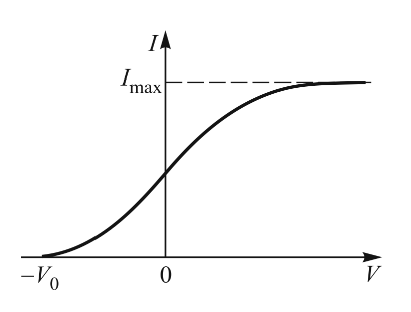
\includegraphics[scale = 0.35]{Screenshot 2023-09-06 at 9.50.13 AM.png}
\caption{Зависимость фототока от напряжения на аноде фотоэлемента}
\label{ris:1}
\end{wrapfigure}
\section{Теоретический материал \cite{1}}
Испускание электронов фотокатодом, облучаемым светом, называется внешним фотоэфектом. Такое взаимодействие можно представить как столкновение фотонов, несущих энергию $\hbar \omega$ и импульс $\hbar \omega /c$, и электронов фотокатода. Энергетический баланс фотоэффекта описывается уравнением 
\begin{equation}
    \hbar \omega = E_{max} + W
    \label{enbalance}
\end{equation}
где  $E_{max}$ - максимальная кинетическая энергия электрона после выхода из фотокатода, $W$ - работа выхода электрона из катода.


Для измерения энергии вылетевших фотоэлектронов (реально их энергетический спектр непрерывен - он простирается от 0 до $E_{max}$) вблизи фотокатода располагают анод, на который подается задерживающий ($V$<0) или ускоряющий ($V$>0) потенциал.

При достаточно больших ускорящий напряжениях фототок достигает насыщения (рис.\eqref{ris:1}) : все испущенные электроны попадают на анод, а при задерживающих потенциалах электроны с малой кинетической энергией заворачиваются полем и не достигают анода. При некотором значении $V = -V_0$ - потенциале запирания - фототок достигает нуля. 

Для потенциала запирания верна свзяь с максимальной кинетической энергией электронов 
\begin{equation}
    E_{max} = e\cdot V_0
    \label{Emax}
\end{equation}

Подставив \eqref{Emax} в \eqref{enbalance} получим \textbf{уравнение Эйнштейна для фотоэффекта} : 
\begin{equation}
    e\cdot V_0 = \hbar \omega - W
    \label{einstaein}
\end{equation}

Чтобы определить величину запирающего напряжения, нужно правильно экстраполировать получаемую токовую зависимость рис. \eqref{ris:1} к нулю. Для поиска функциональной зависимости $I(V)$ по рассчету для простейшей геометрии - плоского катода, освещаемого светом и параллельного ему анода приходим к зависимости 
\begin{equation}
    \sqrt{I} \propto (V_0- V)
    \label{I = V0-V}
\end{equation}

\begin{wrapfigure}{r}{0.3\textwidth}
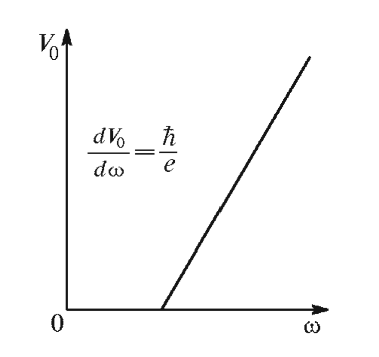
\includegraphics[scale = 0.3]{Screenshot 2023-09-08 at 11.04.24 AM.png}
\caption{Зависимость запирающего потенциала от частоты света}
\label{ris:2}
\end{wrapfigure}


С целью экспериментальной проверки уравнения Эйнштейна \eqref{einstaein} в работе определяются потенциалы запирания $V_0$ для различных частот света $\omega$, лежащих в видимой области спектра. Затем строится зависимость $V_0(\omega)$, которая, согласно \eqref{einstaein}, имеет вид
\begin{equation}
    V_0 = \frac{\hbar \omega - W}{e}
    \label{V0(w)}
\end{equation}

Поэтому по наклону прямой на графике $V_0(\omega)$ (рис. \eqref{ris:2}) можно определить постоянную Дирака:
\begin{equation}
    \frac{dV_0}{d\omega} = \frac{\hbar}{e}
    \label{def h}
\end{equation}

Как показывает формула \eqref{def h}, угол наклона прямой $V
_0(\omega)$ не зависит от рода вещества, из которого сделан катод. Но от рода зависит величина фотопотока и работа выхода $W$ и форма кривой $I(V)$. Все это определяет выбор пригодных для опыта катодов.

\section{Экспериментальная установка}
\begin{figure}[h!]
    \centering
    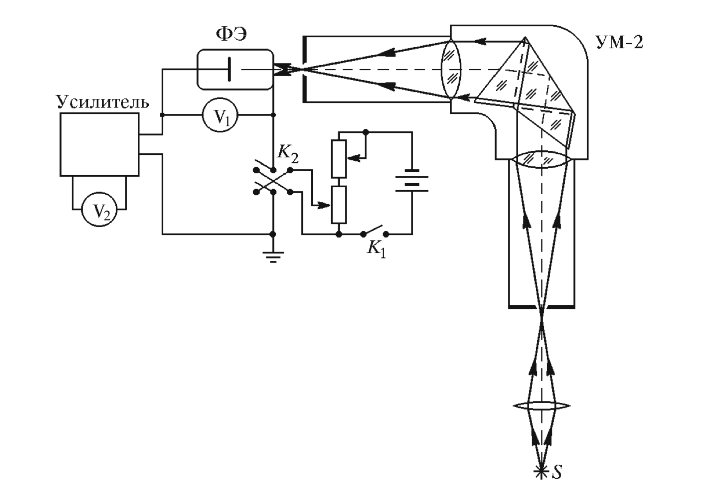
\includegraphics[scale = 0.4]{Screenshot 2023-09-08 at 11.24.59 AM.png}
    \caption{Принципиальная схема экспериментальной установки}
    \label{fig:3}
\end{figure}


    
Схема установки показана на рис. \eqref{fig:3}. Свет от обычной лампы накаливания с помощью конденсора фокусируется на входную щель призменного монохроматора УМ-2, выделяющего узкий спектральный интервал, и попадает на катод фотоэлемента ФЭ. 

Фотоэлемент представляет собой откачанный до высокого вакуума стеклянный балон, с расположенными внутри фотокатодом и анодом, где фотокатод - тонкая пленка металла, легированная элементами $Na, ~K, ~Cs$, расположенная на массивной металлической пластине, а анод выполнен в виде пояска тонкой пленки, осажденной на внутренней части боковой поверхности вверху балона. Наибольшая чувствительность ФЭ лежит в области от 400 до 500 нм, а полная область чувствительности - от 300 до 850 нм. 

Абсолютные значения фототока нам не нужны, поэтому он измеряется в относительных единицах цифровым вольтметром $V_2$, подключенным к выходу усилителя постоянного тока. Эти показания пропорциональны величине измеряемого тока. Тормозящий потенциал регулируется при помощи двух потенциометров "Грубо" и "Плавно". Измерение тормозящего потенциала осуществляется с помощью вольтметра $V_1$. 
\newpage{}
\section{Результаты измерений и обработка данных}

\subsection{Градуировка монохроматора}
\begin{enumerate}


\item Используя зрительную трубу монохроматора, проградуируем барабан монохроматора по спектру неоновой лампы и построим соответствующую градуировочную кривую (рис. \eqref{grapcurv}).
\begin{figure}[h!]
    \centering
 
    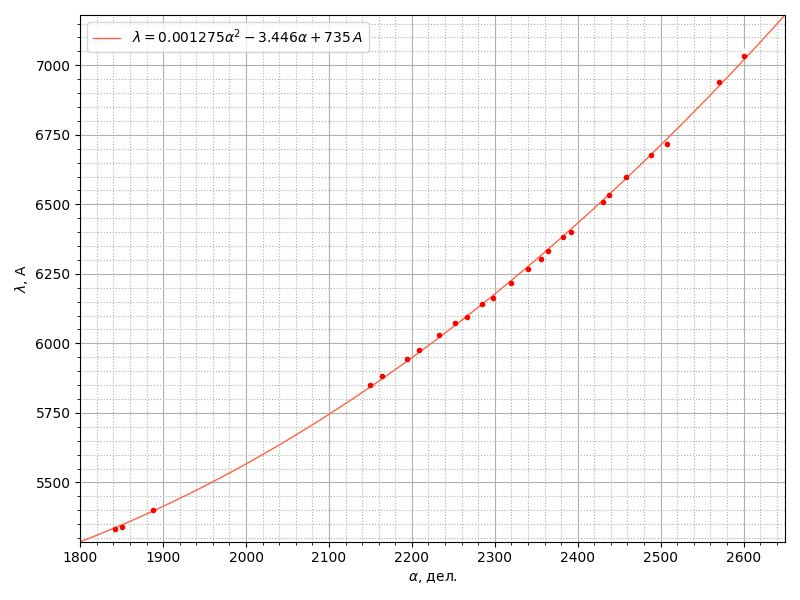
\includegraphics[scale = 0.5]{photo_2023-09-10 3.28.19 PM.jpeg}
    \caption{Градуировочная кривая монохроматора}
    \label{grapcurv}
\end{figure}

%\item Для слеюдующего пункта нам нужно выбрать 7-9 значений углов на барабане, соответствующих длинам волн из диапазона от 540 до 700 нм. Мы это сделали с шагом в 50 градусов от $\alpha = 2150^{o}$ до  $\alpha = 2500^{o}$. 

\item Проведем аппроксимацию градуировочной кривой полиномом второй степени по МНК:
\begin{equation*}
    \lambda = 0.00128 \alpha^2 - 3.446 \alpha + 7358 \text{ A}
\end{equation*}

\begin{equation*}
    a = (12.8 \pm 0.4)\cdot 10^{-4} \AA; ~~~
    b = -3.45 \pm 0.17 \AA;~~~
c = (73.6 \pm 1.9)\cdot 10^{2} \AA
\end{equation*}
\item Определим погрешность вычисления длин волн и циклических частот ($\omega = 2\pi c/\lambda$):
\begin{equation*}
    \delta \lambda = \sqrt{(f_{\alpha}^{'}  \cdot \delta \alpha)^{2}+ (f^{'}_a \cdot \delta a)^{2} +(f^{'}_b\cdot \delta b)^{2} +(f^{'}_c \cdot \delta c)^{2}}  \approx  \sqrt{(\alpha^2 \cdot \delta a)^{2} +(\alpha \cdot\delta b)^{2} + \delta c^{2}}
\end{equation*}

\begin{equation*}
\delta \omega = |\omega_{\lambda}^{'} | \delta \lambda = \left|\frac{-2\pi c}{\lambda^2}\right |\delta \lambda.
\end{equation*}
\end{enumerate}

\subsection{Исследование зависимости фототока от величины запирающего потенциала}
\begin{enumerate}
 

\item Заменим неоновую лампу на электрическую.

 \item Снимем зависимости фототока от напряжения для выбранных длин волн, меняя V в диапазоне от величины ~ $V_0$, где фототок около нуля, до ~ 0.  Построим серию графиков $\sqrt{I} = f(V)$ (рис. \eqref{fig:seria}), определяя для каждой длины волны величину запирающего потенциала как  $b/a$, где $ax+b$ - прямая, аппроксимирующая полученную кривую (Таблица \eqref{table a,b,V}). 

\begin{figure}[h!]
    \centering
    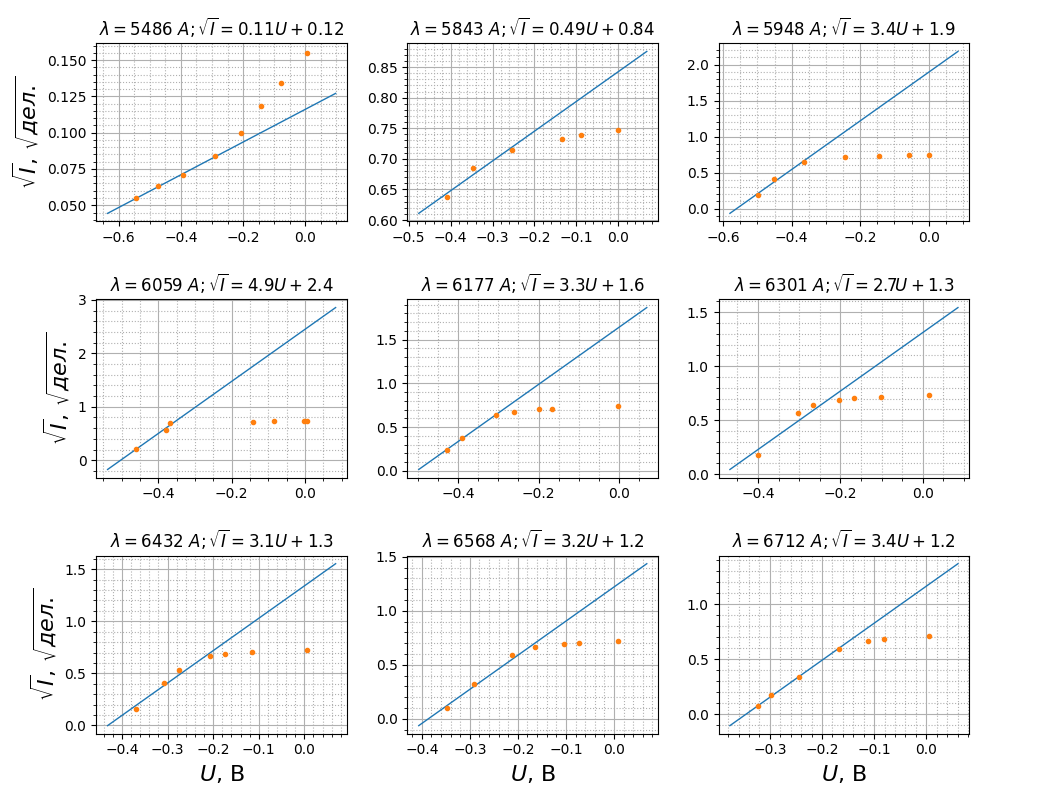
\includegraphics[scale = 0.69]{5.5.1!!.png}
    \caption{Серия графиков $\sqrt{I} = f(V)$}
    \label{fig:seria}
\end{figure}

% Please add the following required packages to your document preamble:
% \usepackage[table,xcdraw]{xcolor}
% If you use beamer only pass "xcolor=table" option, i.e. \documentclass[xcolor=table]{beamer}
% Please add the following required packages to your document preamble:
% \usepackage[table,xcdraw]{xcolor}
% If you use beamer only pass "xcolor=table" option, i.e. \documentclass[xcolor=table]{beamer}



\begin{table}[h!]

\centering
\caption{Коэффициенты аппроксимпации кривых и величины запирающего напряжения для каждой длины волны}
\begin{tabular}{|
>{\columncolor[HTML]{FFFFFF}}c |
>{\columncolor[HTML]{FFFFFF}}c |
>{\columncolor[HTML]{FFFFFF}}c |
>{\columncolor[HTML]{FFFFFF}}c |
>{\columncolor[HTML]{FFFFFF}}c |
>{\columncolor[HTML]{FFFFFF}}c |}

\hline

{$\alpha, ^0$} & {$\lambda,~\text{\AA}\ $} & $a, \frac{\sqrt{A}}{B}$ & $b, \sqrt{A}$ & \textbf{$V_0,~ B$} & $\omega,~10^{15}~\text{ с}^{-1}$\\ \hline






1950           & 5480 $\pm$   410        & 0,106  $\pm$  0,007   & 0,113 $\pm$  0,003    & 1,06  $\pm$    0,08   & 3,4 $\pm$0,3\\ \hline

2150           & 5840  $\pm$   450       & 0,33 $\pm$  0,09    & 0,79 $\pm$  0,03    & 1,7 $\pm$    0,3   & 3,2 $\pm$0,3\\ \hline

2200           & 5950  $\pm$   460       & 3,4 $\pm$  0,6    & 1,9 $\pm$  0,3    & 0,56 $\pm$    0,12   & 3,2 $\pm$0,3\\ \hline

2250           & 6060  $\pm$   470       & 4,8 $\pm$  0,8    & 2,5 $\pm$    0,3  & 0,50 $\pm$     0,11   & 3,1 $\pm$0,2\\ \hline

2300           & 6180  $\pm$    480      & 3,27 $\pm$  0,16    & 1,64 $\pm$   0,06   & 0,50 $\pm$   0,03     & 3,1 $\pm$0,2\\ \hline

2350           & 6300 $\pm$    490       & 3,6 $\pm$   0,4   & 1,63  $\pm$   0,14  & 0,45 $\pm$     0,07   & 3,0 $\pm$0,2\\ \hline

2400           & 6430 $\pm$    500       & 3,1 $\pm$  0,4    & 1,34  $\pm$   0,13  & 0,43 $\pm$    0,07   & 2,9 $\pm$0,2\\ \hline
2450           & 6570 $\pm$   520        & 3,2 $\pm$  0,3    & 1,22   $\pm$  0,09  & 0,39  $\pm$  0,05  &   2,9 $\pm$0,2\\ \hline

2500           & 6710   $\pm$    530     & 3,34 $\pm$  0,05    & 1,16  $\pm$ 0,01    & 0,348   $\pm$  0,007 &  2,8 $\pm$0,2\\ \hline








\end{tabular}
\label{table a,b,V}
\end{table}

\end{enumerate}
\newpage
\subsection{Определение постоянной Дирака, оценка красной границы и работы выхода матриала катода}

\begin{enumerate}


\item  Построим график зависимости $V_0(\omega)$ с помощью взвешенного МНК. Две последние точки не будем учитывать в силу их заметного отклонения от остальных значений и линейной зависимоти :
\begin{equation*}
    a = 0,55 \pm 0,05 \cdot 10^{-15}\text{ c}\cdot \text{ B};~~~b = -1,18 \pm 0,16 \text{ B}.
\end{equation*}

\begin{figure}[h!]
    \centering
    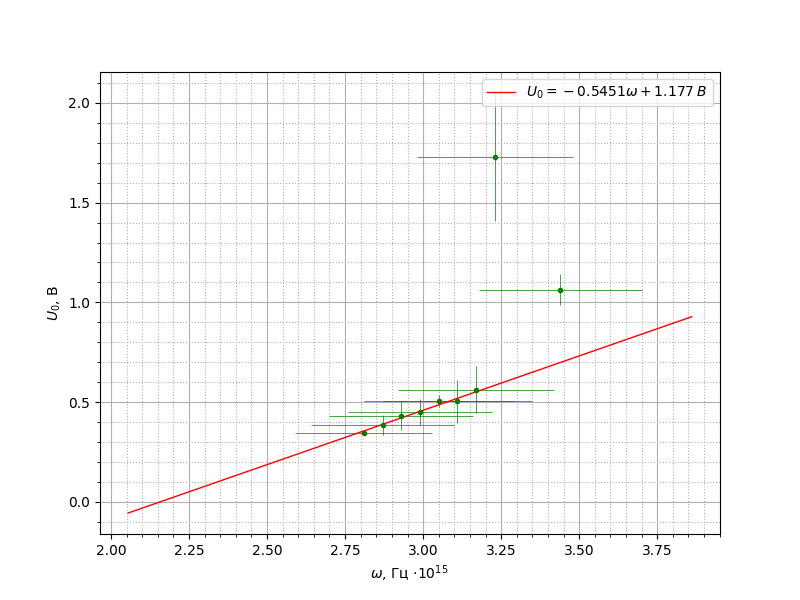
\includegraphics[scale = 0.9]{5.5.1(hhhh).png}
    \caption{График зависимости $V_0(\omega)$}
    \label{fig: h}
\end{figure}


\item Определим по полученным данным значение постоянной Дирака, используя формулу \eqref{def h}:
\begin{equation*}
    \hbar = a \cdot e = 0.55\cdot 10^{-15}\cdot 1.6\cdot 10^{-19} = 0,87 \pm 0.08 \cdot 10^{-34}\text{Дж}\cdot \text{с}.
\end{equation*}
Табличное значение постоянной Дирака: 
\begin{equation*}
    \hbar = 1,055\cdot 10^{-34} \text{Дж}\cdot \text{с}.
\end{equation*}
\item Найдем красную границу фотоэффекта. Для этого определим частоту, при которой потенциал запирания обращается в ноль.
\begin{equation*}
    \omega_{кр} = \frac{-b}{a} = (2,2 \pm 0,3 )\cdot 10^{15} \text{Гц}
\end{equation*}
Соответствующая длина волны:
\begin{equation}
    \lambda_\text{к} = \frac{2\pi c}{\omega} = 860 \pm 120\text{ нм}.
\end{equation}


\item Найдем работу выхода материала катода:
\begin{equation*}
    W = \hbar\cdot \omega_{кр} = (2,3\pm 0,3)\cdot 10^{-19}\text{ Дж} = 1,45 \pm 0,18 \text{ эВ}.
\end{equation*}

\end{enumerate}

\section{Обсуждение результатов и выводы}
\begin{itemize}



 \item Была исследована зависимость фототока от величины задерживающего напряжения: экспериментально проверено,  что квадратный корень из фототока линейно зависит от задерживающего напряжения.

 \item В ходе работы были определены следующие величины:
 
 \begin{enumerate}
     \item  Постоянная Дирака:

\[\hbar_\text{эксп} = 0,87 \pm 0.08 \cdot 10^{-34}\text{Дж}\cdot \text{с}\]
\[\hbar_\text{теор} = 1,055\cdot 10^{-34} \text{Дж}\cdot \text{с}\]

    \item Красная граница фотоэффекта:

\[\lambda_\text{к} = 860 \pm 120\text{ нм}\] 

    \item Работа выхода материала катода:

    \[W = 1,45 \pm 0,18 \text{ эВ}\]
\end{enumerate}
\end{itemize}
\newpage


\addcontentsline{toc}{section}{Список используемой литературы}
\begin{thebibliography}{}
     \bibitem{1} ЛАБОРАТОРНЫЙ ПРАКТИКУМ ПО ОБЩЕЙ ФИЗИКЕ. Квантовая физика: Учеб. пособие для вузов / Игошин Ф.Ф., Самарский Ю.А., Ципенюк Ю.М.; Под редакцией Ципенюка Ю.М. - М. : Физматкнига, 2012 - 464 с. - 
    \bibitem{2}  1.1. Экспериментальная проверка уравнения Эйнштейна для фотоэффекта. Дополнительное описание . Исправлено 1-VII-2011
\end{thebibliography}

\end{document}
